\chapter{User Interface Basics}

\section{User interface components}
\subsection{Widget}
What is a widget? Widget is just a fancy name for user interface element or controller for example button, label, check box etc. There are a lot of widgets available in android. In the design mode, if you look at the left side panel called the ``Palette panel'', you would see all of the UI controls or widgets that you can use in your app:

\begin{center}
	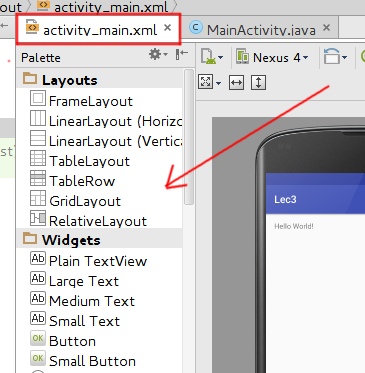
\includegraphics[scale=0.4]{chapters/ch03/images/1_palette_panel}
\end{center}

\subsection{Basic concepts}

\subsubsection{Views}
In android a ``\texttt{View}'' is an interact-able rectangle on the screen. Just like the concept of windows, everything is a window in Windows operating system, pretty much everything is a view in android. So the buttons, text labels, text fields, radio buttons etc all are views. There is actually a class in the android SDK called ``\texttt{View}'' and every widget is inherited from it. For more details on the \texttt{View} class refer to the following link:

\url{https://developer.android.com/reference/android/view/View.html}\\

\underline{\textbf{Very important:}} Unlike windows operating system, a view CAN NOT contain other views in it.

\subsubsection{View groups}
``\texttt{ViewGroup}'' is a \textit{special} type of \texttt{View} (actually it is inherited form the ``\texttt{View}'' class available in android SDK). A view group is a container that can contain other \texttt{Views} or even \texttt{ViewGroups} (these are called ``children''). By building up a hierarchical structure like this you can form very complex user interfaces with ease as shown below:

\begin{center}
	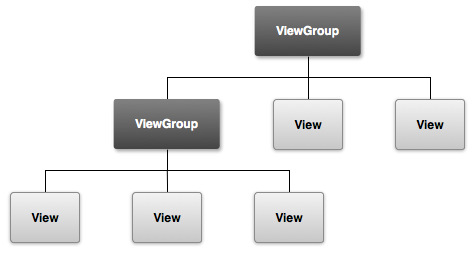
\includegraphics[scale=0.4]{chapters/ch03/images/2_viewGroups}
\end{center}

We have a \texttt{ViewGroup} class in android that is inherited from \texttt{View} class. For more details on the \texttt{ViewGroup} class refer to the following link:

\url{https://developer.android.com/reference/android/view/ViewGroup.html} \\

\underline{Usage:} Some examples of view groups include the \texttt{RelativeLayout}, \texttt{LinearLayout}, \texttt{FrameLayout}, \texttt{GridLayout}, \texttt{Fragments} etc. Generally the view groups are used to contain other widgets and to format or display them nicely on the screen. \\

\underline{\textbf{Very important fact:}} Your app MUST have AT LEAST \underline{ONE} \texttt{ViewGroup} on top (head) of the UI hierarchy. By default when you create a new project the root is set to ``\texttt{RelativeLayout}''.\\

Ok, let's see all of this in action.

\subsection{Widgets and containers in detail}
\subsubsection{Create new project}
\label{sec:createProj}

To complete this class activity let's start fresh and create a new project from scratch. Perform the following steps:
\begin{enumerate}
	\item Create a new project having name ``\texttt{Lec3}''
	\item Select minimum API 16 : Android 4.1 (Jelly Bean).
	\item Select ``\texttt{Empty Activity}''
	\item Accept default values for activity and finish.
\end{enumerate}

\subsubsection{Linear Layout}
Assuming that you've chosen default names, open up the layout file ``\texttt{activity\_main.xml}'' and go to the text mode. Right click on the gray colored gutter on the left side and select ``Show line numbers'':

\begin{center}
	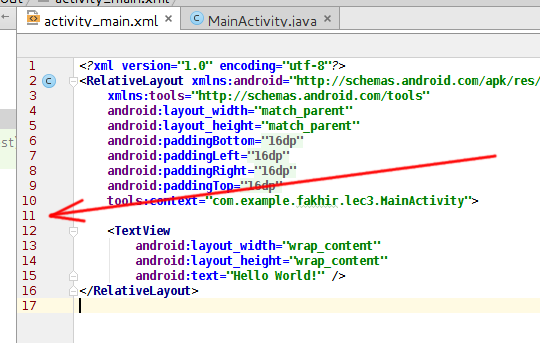
\includegraphics[scale=0.4]{chapters/ch03/images/3_line_numbers}
\end{center}

Go to line 1 and change ``\texttt{RelativeLayout}'' to ``\texttt{LinearLayout}''. Now select and delete lines 6-9. These are the layout attributes or properties. We will look into these in detail later on. Also delete the entire \texttt{TextView} element (lines 8-11). You should have an empty linear layout:

\begin{center}
	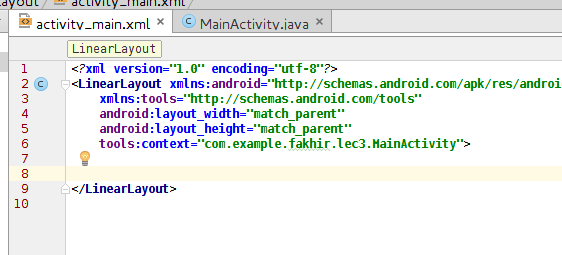
\includegraphics[scale=0.4]{chapters/ch03/images/4_linear_layout}
\end{center} 

\underline{\textbf{\texttt{LinearLayout:}}} A linear layout is a view group. It is inherited from the \texttt{ViewGroup} class. This means that it is a container that can contain buttons, labels etc and even other liner layouts ! A linear layout displays its children in either a horizontal or a vertical arrangement.

Go to th design mode and drag two widgets on top the linear layout as shown below:

\begin{center}
	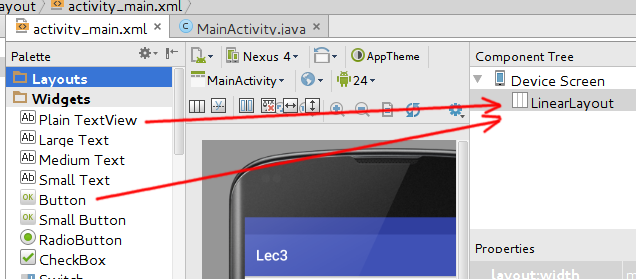
\includegraphics[scale=0.4]{chapters/ch03/images/5_linear_layout}
\end{center} 

Once you've added the widgets to the layout, click to select the ``Linear Layout'' root element from the component tree panel. Change its ``\texttt{orientation}'' property to horizontal. 

Once you've done that, now try changing the orientation to ``vertical'':

\begin{center}
	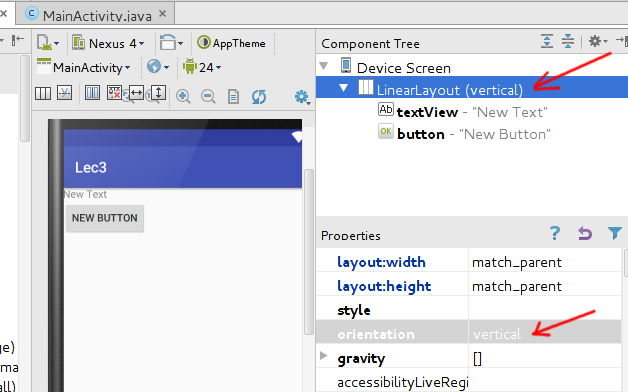
\includegraphics[scale=0.4]{chapters/ch03/images/6_linear_layout}
\end{center} 

Verify that the changes have been correctly updated in the preview panel.\\

Change the label text to ``Hello World !!!'' and button text to ``Click me''. Notice that even though we used mixed case string in both cases but the actual output string on the button is all caps:

\begin{center}
	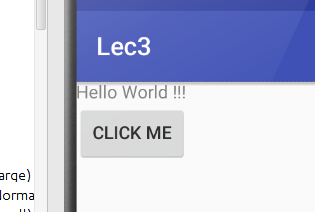
\includegraphics[scale=0.4]{chapters/ch03/images/7_change_text}
\end{center} 

If you want to change this to mixed caps, then switch to text mode. In ``activity\_main.xml'' find the button element. Add an attribute named ``\texttt{android:textAllCaps}'' and set it to \texttt{false}. The preview window will update automatically to reflect the changes:

\begin{center}
	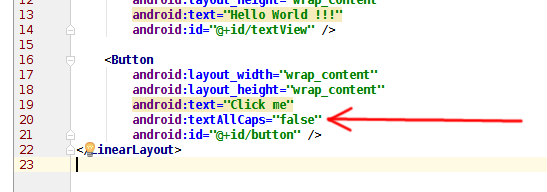
\includegraphics[scale=0.4]{chapters/ch03/images/8_text_case}
\end{center} 

Switch to the design mode and try setting the \texttt{textAllCaps} attribute for our text label to \texttt{true}. \\

You can read more about linear layouts here:

\url{https://developer.android.com/guide/topics/ui/layout/linear.html}

\subsubsection{View dimensions}

While in design mode, from the preview panel in the middle, click on the text label named ``Hello World !!!''. A blue rectangle will appear around it. This blue rectangle shows the current size of that widget. Let's try to change the width of this text view. While text view still selected, on the right side properties panel you should see the ``\texttt{layout:width}'' attribute with a value of ``\texttt{wrap\_content}''. \texttt{wrap\_content} tells the widget to set its width to the smallest size just to contain all of its children. The only child of text view is that text, to the size of the entire controller is adjusted according to that, just like a rubber band wrapped around a bunch of pencils. Thy changing the text to something long and see how the size of the widget changes.

\begin{center}
	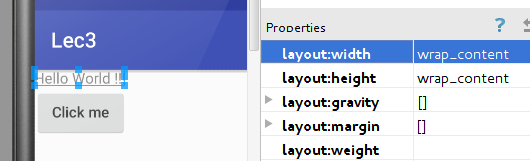
\includegraphics[scale=0.4]{chapters/ch03/images/9_layout_width}
\end{center} 

With text view still selected, change the ``\texttt{layout:width}'' to ``\texttt{match\_parent}''. \texttt{match\_parent} tells the widget to adjust its size to match its parent's size as much as possible (if there are no other widgets in the way). Its like inflating a big-balloon inside a small container. Watch the new size of our text view change to match the boundaries of the phone itself.

\begin{center}
	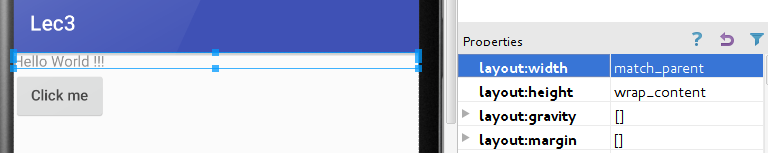
\includegraphics[scale=0.4]{chapters/ch03/images/10_layout_width}
\end{center} 

Try to change the orientation of the device to landscape, you will see that the text view changes its size automatically to match its parent. 

\subsubsection{View Gravity}

Now let's explore some other attributes. Change the ``\texttt{layout:width}'' of the text view back to \texttt{wrap\_content}. Also change the \texttt{background} color to something you like so that we can see its exact size against the white canvas. Find and expand the attribute named ``\texttt{layout:gravity}''. Check the ``right'' field. The text view will snap to the right edge of the screen:

\begin{center}
	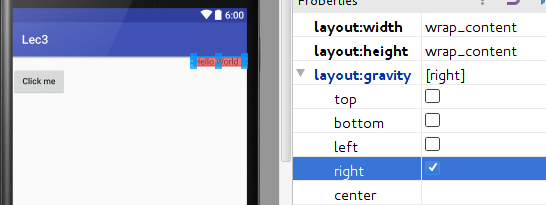
\includegraphics[scale=0.4]{chapters/ch03/images/11_layout_gravity}
\end{center} 

Uncheck ``right'' and click on the ``center'' field, then select ``horizontal'' and see what happens. \\

\underline{\textbf{Note:}} When you are setting \texttt{layout:gravity} the view needs some space to move around or to set its position. If the view doesn't appear to change its position, check the size of its parent. Is the parent big enough to allow the child to move around inside it? \\

After this, now click on the button to select it. Try changing its position through \texttt{layout:width}. Apart from \texttt{layout:gravity} each view also has a separate attribute called \texttt{gravity}. This changes the position of its \textit{``children''}. For example it you set the \texttt{gravity} field of the button to both ``bottom'' and ``center'' the text of the button (which is the child of the button view) will move towards the bottom edge of the button. Optionally also set the \texttt{layout:height} (the height of the button) to 70dp:

\begin{center}
	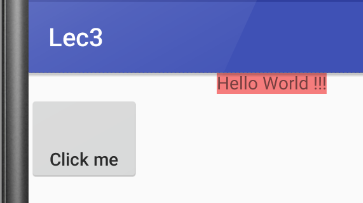
\includegraphics[scale=0.4]{chapters/ch03/images/12_gravity}
\end{center} 

\underline{\textbf{Important distinction:}}\\

\textbf{\texttt{layout:gravity}} $\rightarrow$ Sets the position of the current view inside its parent.

\textbf{\texttt{gravity}} $\rightarrow$ Sets the position of all the children inside the current view (or view group). \\

\subsubsection{Margin and Padding}
As an extra step select the linear layout and change its background to something yellowish. Also change both of its \texttt{layout:width} and \texttt{layout:height} to \texttt{wrap\_content}. \\

\textbf{``Margin'':} It defines how much gap there is between two views (or view groups). If the views don't have any margins around them they will bump into each other. 

\begin{center}
	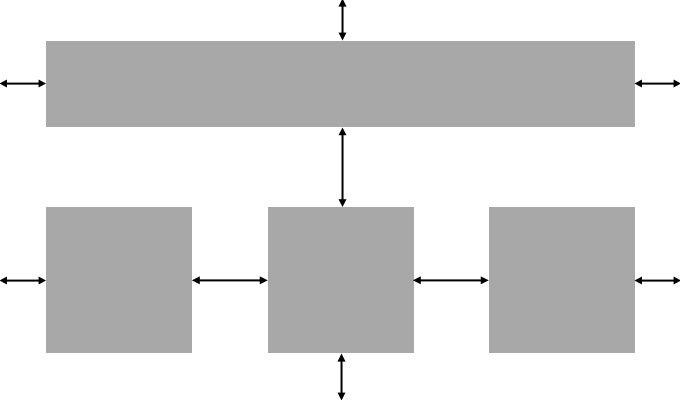
\includegraphics[scale=0.2]{chapters/ch03/images/13_margin_def}
\end{center} 

Select text view again and look for ``\texttt{layout:margin}'' attribute. Change the ``all'' field to \texttt{10dp}. You will notice that there is now a gap of 10 points all around the text label. You can also set the margin individually for each of the view sides. 

\begin{center}
	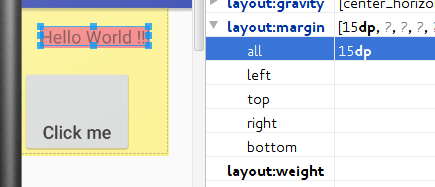
\includegraphics[scale=0.4]{chapters/ch03/images/14_margin}
\end{center} 

\textbf{``Padding'':} This increases te size of the control. Imagine wrapping a box with a very thick foam. 

\begin{center}
	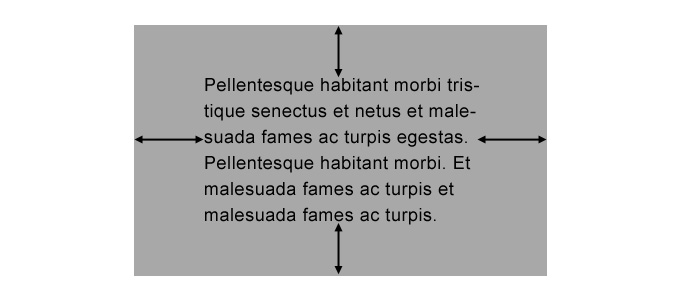
\includegraphics[scale=0.2]{chapters/ch03/images/15_padding_def}
\end{center}

Select text view again and look for ``\texttt{padding}'' attribute. Change the ``all'' field to \texttt{10dp}. You will notice that text view got a bit bigger:

\begin{center}
	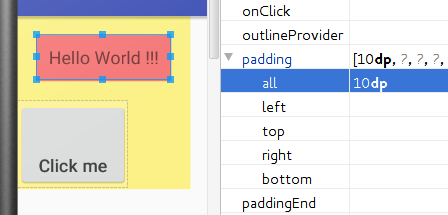
\includegraphics[scale=0.4]{chapters/ch03/images/16_padding}
\end{center}

You can do this with any view or control to customize its outlook.

\underline{\textbf{To summerize:}}

\textit{\textbf{Margin:}} Between border and its parent layout

\textit{\textbf{Padding:}} Between content and border

\begin{center}
	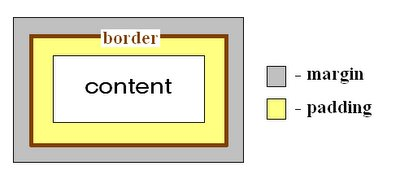
\includegraphics[scale=0.3]{chapters/ch03/images/17_mar_pad}
\end{center}

\subsubsection{Modifying the XML}
Sometimes our required attributes are not present in the design view. To see this, switch to design mode and select linear layout. From the properties panel try to find attributes named ``\texttt{layout:gravity}''. You won't be able to find it. 

Now time to edit some XML, switch to the text mode. Add an attribute named \texttt{layout:gravity} in the \texttt{LinearLayout} element and set it to ``center'':

\begin{center}
	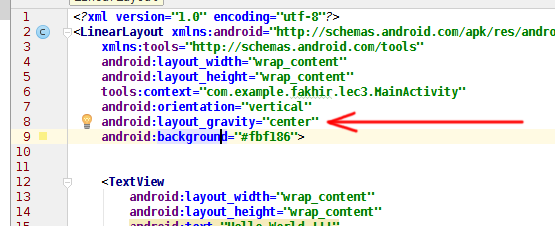
\includegraphics[scale=0.4]{chapters/ch03/images/18_ll_grav}
\end{center}

Once you've done that, the preview window will automatically update to reflect changes:

\begin{center}
	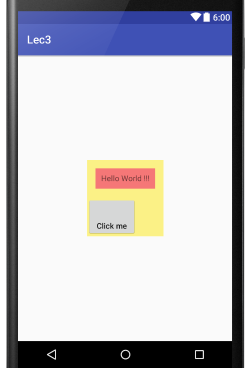
\includegraphics[scale=0.3]{chapters/ch03/images/19_output}
\end{center}

\textit{Tip:} You can exclusively use text mode without ever having to go to the design mode.

\subsection{A bit complex example}
Follow the steps in \hyperref[sec:createProj]{section 1.3.1} create a new project. You can name it something like ``Lec3b'' or ``ClassAssign2'' etc. \\

Go to the text mode, change the layout to linear. Also delete the text view. Make sure that the root layout is empty. Now switch to design mode. Select the \texttt{LinearLayout} from component tree and set its \texttt{orientation} to ``vertical''. Also make sure
that the gravity is unset:

\begin{center}
	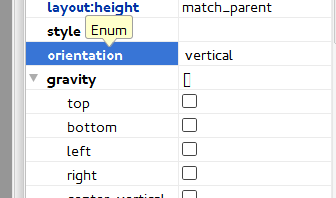
\includegraphics[scale=0.4]{chapters/ch03/images/20}
\end{center}

Now drag a new \texttt{LinearLayout} (horizontal) from the control palette on the left and drop it on top of the parent \texttt{LinearLayout} inside component tree:

\begin{center}
	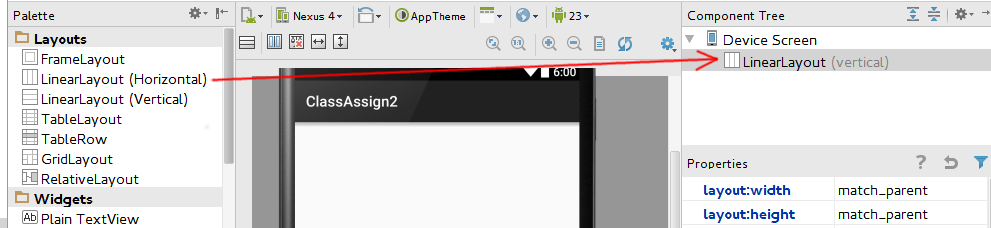
\includegraphics[scale=0.4]{chapters/ch03/images/21}
\end{center}

Select the child linear layout and set its \texttt{layout:height} to ``\texttt{wrap\_content}'':

\begin{center}
	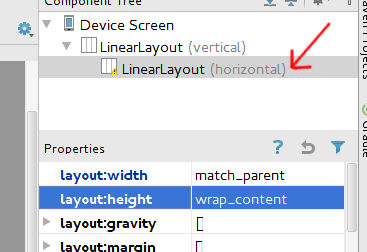
\includegraphics[scale=0.4]{chapters/ch03/images/22}
\end{center}

Drag ``Large Text'' view on top of the child \texttt{LinearLayout}. Set its text to ``Hello !!! This is a test label.'':

\begin{center}
	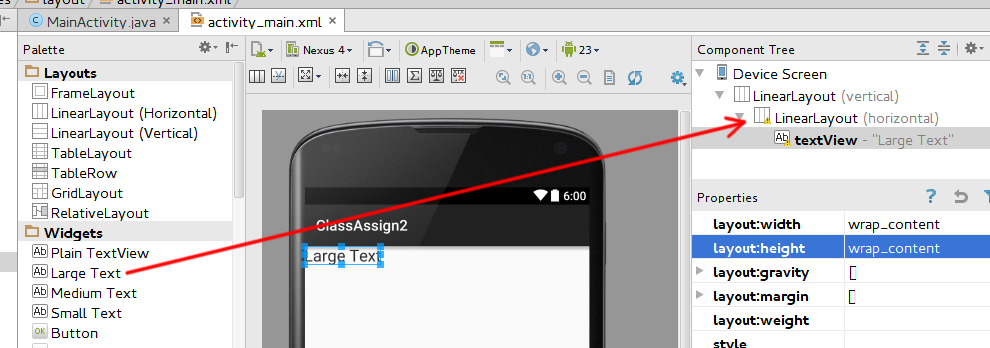
\includegraphics[scale=0.4]{chapters/ch03/images/23}
\end{center}

Drag an \texttt{imageView} on top of child \texttt{LinearLayout}. Change its \texttt{src} parameter to \texttt{@mipmap/ic\_launcher}:

\begin{center}
	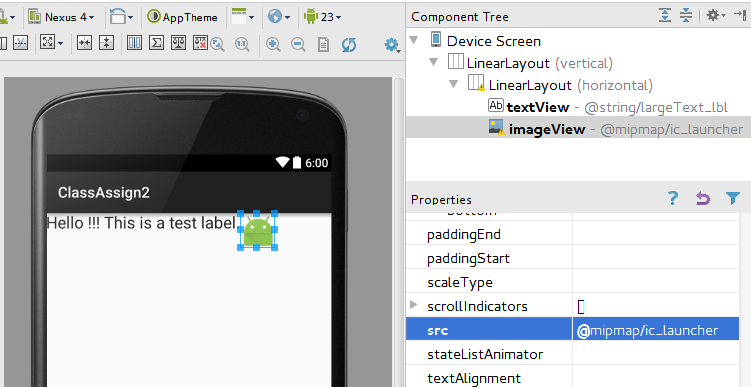
\includegraphics[scale=0.4]{chapters/ch03/images/24}
\end{center}

Go to the text mode and make sure that the preview window is visible. In the xml file, as soon as you place your keyboard cursor on the \texttt{LinearLayout} tag, the layout will be highlighted in the right preview window:

\begin{center}
	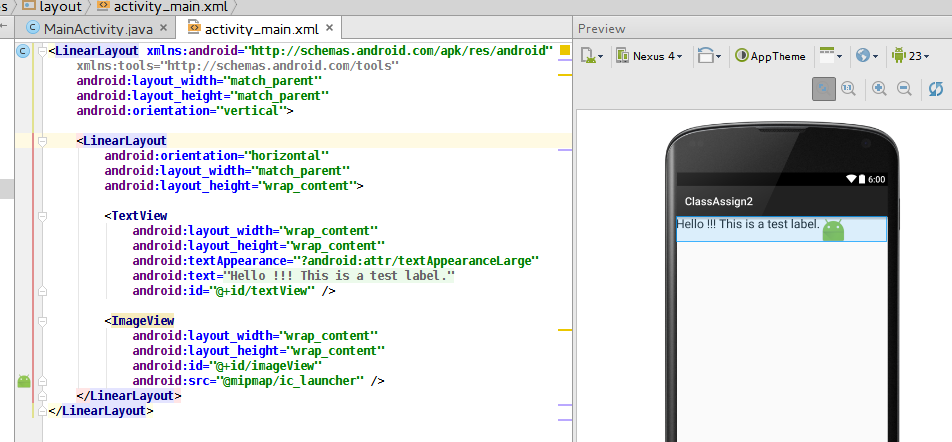
\includegraphics[scale=0.4]{chapters/ch03/images/25}
\end{center}

Remember the gravity parameter arranges the contents inside a view? Go back to the design mode, select the child linear layout and set its \texttt{gravity} to ``\texttt{center\_horizontal}'':

\begin{center}
	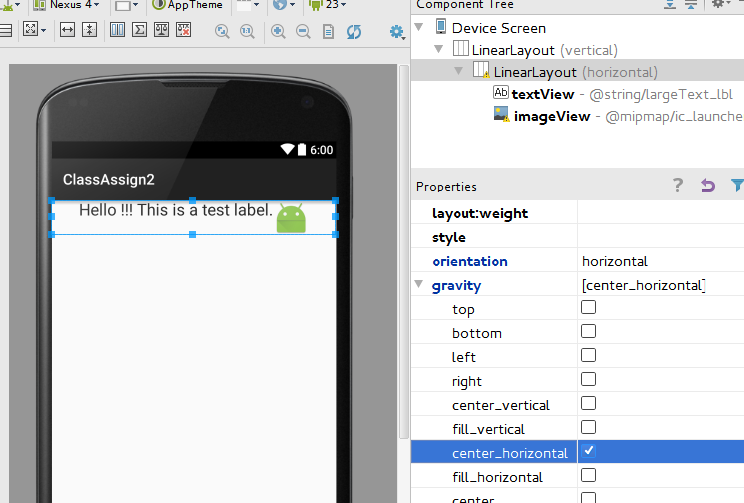
\includegraphics[scale=0.4]{chapters/ch03/images/26}
\end{center}

As we saw earlier that \texttt{layout:gravity} decides how a view is positioned inside a parent. We want the green android image to be right justified. Click on the image view and set its \texttt{layout:gravity} to right. \\

Hmmm, nothing appears to happen !!!

\subsection{Simple Task}
Continuing from the example above:

\begin{enumerate}
	\item Go to the design view. Wrap the image view inside a \texttt{LinearLayout} (vertical). Now try adjusting
	the \texttt{layout:gravity} of the \texttt{imageView} and see if it adjusts itself!
	\item Alternatively you can set the gravity of the \texttt{LinearLayout} to ``right'' yielding the same result. Two
	different ways to do the same thing!
\end{enumerate}

\section{Exercises}
\subsection{Layout 1:}
Produce an output similar to the following:
\begin{center}
	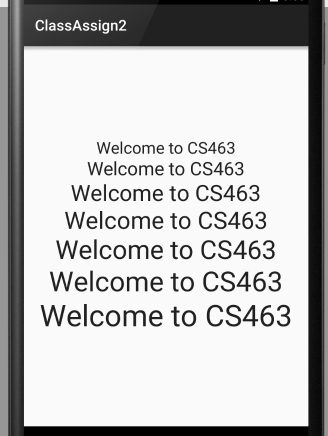
\includegraphics[scale=0.4]{chapters/ch03/images/27}
\end{center}

\subsection{Layout 2:}
Produce an output similar to the following. You can achieve this by combining various orientations of linear layouts:

\begin{center}
	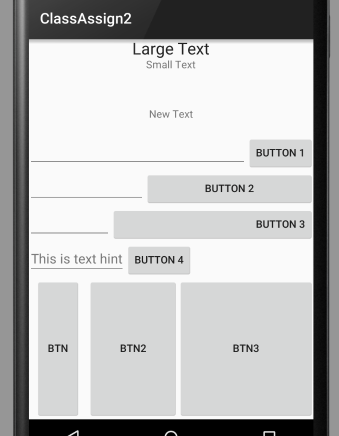
\includegraphics[scale=0.4]{chapters/ch03/images/28}
\end{center}

\textit{\textbf{Warning:}} Hint on the next page.

\newpage
\subsection{Hint:}
Combination of linear layouts. First try to draw view hierarchy tree on a piece of paper. You are completely free to exclusively use \texttt{RelativeLayout} as well!

\begin{center}
	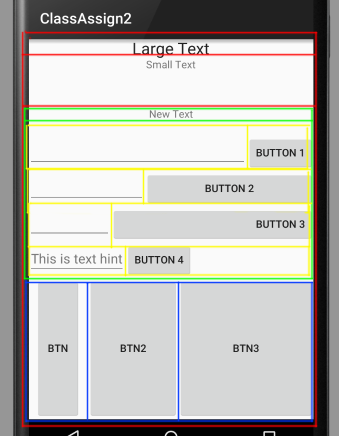
\includegraphics[scale=0.45]{chapters/ch03/images/29}
\end{center}

\section{Homework}
Investigate about the view attribute named ``\texttt{weight}'' and do some practice with it. You can read about it from here:

\begin{enumerate}
	\item \url{https://developer.android.com/guide/topics/ui/layout/linear.html#Weight}
	
	\item \url{http://android.amberfog.com/?p=328}
	
	\item \url{http://www.101apps.co.za/index.php/articles/using-android-s-layout-weight-attribute.html}
\end{enumerate}